\section {K-fold cross validation}%TODO explain in more detail (give pictures)
\subsection{Theory}
In this type of cross validation the data is split into k-subsets and the validation set approach is repeated k times as in the Figure \ref{fig:5-flod}. The cross validation will then be performed using each of the k subsets as the validation set and the other k-1 sets are combined and used as the training set. This method has several advantages over simple cross validation as there is less variance in the test error estimate without being much more computationally complex, only requiring the learning method to be run K times. The cross validation parameter is given by calculating the average MSE for each fold as seen in Formula \ref{fo:k-fold}. 

\begin{figure}[H]
	\centering
	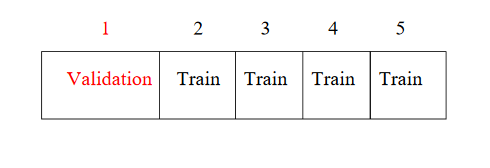
\includegraphics[width=0.5\linewidth]{crossValidation/5-foldCV}
	\caption{5-Fold cross validation}
	\label{fig:5-flod}
\end{figure}

An important aspect of K-fold cross validation is the selection of the k parameter, in practice $k=5$ or $k=10$ is sufficient, as higher values of k tend to lead to unnecessary increases in computation time, as the return on increasing K starts to drop drastically. It does have several advantages over similar cross validation methods, regarding bias/variance trade-offs as K-fold cross validation usually gets less varied results than simple validation set, as it averages several data points, instead of only using a single observation. On the other end of the spectrum is has more bias than Leave One Out Cross Validation as LOOCV averages a large number of highly correlated data points resulting very large bias towards the training set. Leave One Out Cross Validation is s special case of K-fold CV will be discussed in the following chapter where K = n.

\begin{align}\label{fo:k-fold}
CV_{(K)} = \sum_{k=1}^{K}  \frac {n_{k}}{n}MSE_{(k)}
\end{align}

\subsection{Result}
\subsubsection*{LAB 5.3.3}%TODO write full lab
In lab 5.3.3 the objective is to use K-fold validation to get a better estimate for the MSE in the Auto dataset. For the estimate $K=10$ will be used and the results of each run tallied, and in the end $R^2$ and MSE were derived.

Import data and mark the column horsepower as X and mpg as y. Then split the data into 10 folds.
\begin{lstlisting}[language=Python]
('Splits: ', 10)
\end{lstlisting}

Then each fold will be left out in turn, and the model fit 10 times and the results stored. After all 10 runs the MSE and $R^2$ can be estimated.

\begin{lstlisting}[language=Python]
R^2: 54.87992%, MSE: 27.41619
\end{lstlisting}

